\documentclass[11pt]{article}
\usepackage{graphicx}
\usepackage[T1]{fontenc}
\usepackage{txfonts}
\setcounter{secnumdepth}{0}
\usepackage[affil-it]{authblk}   % author affiliation
\usepackage{lineno} %line numbers
\usepackage[a4paper, total={6.5in, 8.5in}]{geometry} % set page size
\usepackage{setspace}

\begin{document}

\title{Demographic Bias in Human Cell Studies }
\author{Jessica Snyder\textsuperscript{1}, Iva Bojic\textsuperscript{1,2}, Aarom Gerow\textsuperscript{3}, Carlo Ratti  \textsuperscript{1,2 } \\ \textsuperscript{1}Massachusetts Institute of Technology, SENSEable City Lab \\ \textsuperscript{2}Singapore-MIT Alliance for Research and Technology \\  \textsuperscript{3}University of Chicago, Computation Institute }

\maketitle 

More than 50,000 woman will be diagnosed with breast cancer between 2010-2020, costing an estimated \$48 billion in medical treatment \cite{mariotto2011projections, weir2015past}. The National Institutes of Health (NIH) and the National Cancer Institute (NCI) invested a combined \$4.1 billion in breast cancer research from 2012 through 2014, with the goal of restoring the nation's breast cancer patient population to good health. With a stable and improving health care system, breast cancer survival rates are at a record high --- more than 90\% --- increasing each year Center for Disease Control (CDC) statistics are available. 

The modern paradigm in cancer research has established that many sub-types of breast cancer are unique pathologies. This motivates using specific traits of the tumor as well as the patient's genetics to make treatment decisions. As the medical community pivots towards increasingly personalized care based on genetic markers, we reflect on the inertia of breast cancer research. After acknowledging that new genomic techniques change how we group patients, lets consider past use of ethnic groups. 

Before gene sequencing was widely available, the CDC grouped the US breast cancer patient population by ethnicity, to identify who might be left out of improving health care options. The purpose was to expand healthy lifestyle choices, public awareness, diagnostics, and treatment options to include considerations of non-majority patients. Here, we use the CDC ethnic groups to assess how well each group has been represented in the available bank of human cell lines and publication that use those cell lines. The breast cancer patient population grouped by CDC-defined ethnicities includes Asian, Black, Hispanic, American Indian and White. The more than 230k US women diagnosed with breast cancer are grouped by ethnicity, and show that breast cancer patients are predominantly white women, 190k or 83\% of the entire incidence population. Black patients comprise 12\% of the incidence population and the remaining 5\% include Asian, Hispanic and Native American women. The incidence rate of breast cancer among White woman has been decreasing since 1999, while the rate among Black and Asian women has increased since 1999 (Figure 1A).

\begin{figure}[h!]
  \centering
  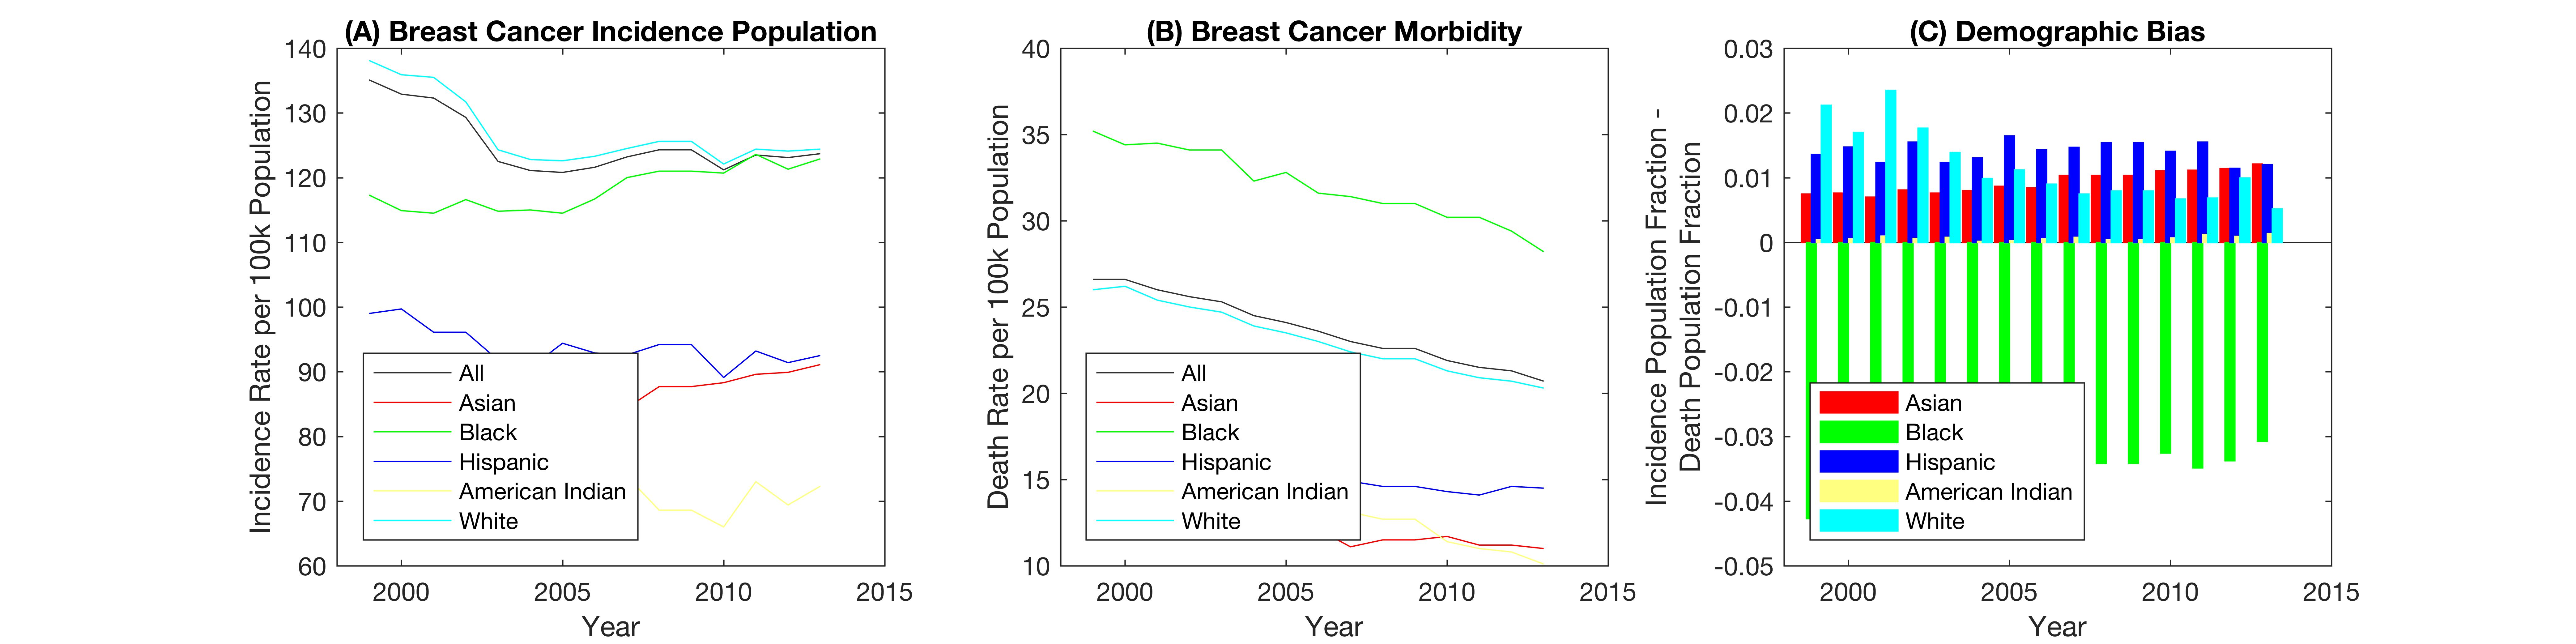
\includegraphics[width=1\columnwidth, trim = {20cm 0cm 10cm 0cm}, clip]{Figures/Rationale.jpg}
  \caption{\label{PS1} Incidence, morbidity and bias in US breast cancer population by ethnicity from 1998-2013. }% Representation in cell models derived from black patients in breast cancer research based on a persistent discrepancy in breast cancer treatment efficacy for black patients.}
\end{figure}

One ongoing success is the steadily declining morbidity for all patients since 1999 (Figure 1B). The CDC statistics, however, shows that Black patients face the worst prognosis for survival after diagnosis. Black patients comprise more of the death population than the incidence: the incidence population fraction is less than the death population fraction (Figure 1C). Black patients are less likely to survive than others, highlighting an acknowledged disparity in the efficacy of breast cancer treatment for black women \cite{greenlee2000cancer, berkman2014racial}. Surprisingly, when the fractions of each ethnicity in the incidence population are compared to the death population, black patients' fraction increase, meaning more black woman die after a breast cancer diagnosis than other ethnicities. Black patients comprise more of the death population than the incidence, the incidence population fraction is less than the death population fraction, figure 1C. White woman comprised the same 83\% of the death population as they did the incidence population, while Asian, Hispanic and Native American fractions decrease slightly. Breast cancer treatment is less effective in treating blacks than all other races. 

Raising the survival rate of Black breast cancer patients to the national average requires critical review of societal, behavioral and biological factors, broadly categorized as societal or extrinsic factors (largely the responsibility of policy research) and the biological, intrinsic factors such as genetics and cell structure within tumor sub-types (largely the responsibility of medical researchers and clinicians) \cite{reding2012examination, brennan2012there}. Socioeconomic-dependence of high-quality health care access and inclusive diagnostic techniques are important without question \cite{shavers2003racial}. Failing to diagnosis at early stages, as well as faster growing, more aggressive tumor sub-types, disproportionately effect black patients \cite{batina2013variation}. This disparity is attributal to a mixture of extrinsic and intrinsic problems affecting black women. Could it be due to access to medical care? Yes. Might it also explained by bias in medical research? Possibly. Here, we review breast cancer research tools and their representation in research publications.

Data-driven analyses of disease burden and treatment effectiveness have been used in the past to guide medical research funding and health policy decisions towards the most productive population-level outcomes \cite{kim2016cancer}. Vetting the influence of intrinsic factors of breast cancer is critical to guide the action of fundamental medical research, and in particular, the demographics of cell lines used in foundational research. Are there intrinsic factors of the tumor sub-types causing morbidity, which are disproportionately present in in black breast cancer patients? Environmental exposure and genetic background determine the a cancer's subtypes, aggressiveness, and ultimately, patient prognosis. Highly aggressive tumor subtypes are correlated to risk factors such as obesity, which disproportionately effects black women. Self-reported race correlated to breast cancer properties, such as estrogen receptor status and stage of diagnosis, more than <XX???XXX> percent African ancestry, suggesting social determinants shape the disease physiology more than genetic predispositions \cite{reding2012examination}. Currently, alternative treatment options for patients with a genetic predisposition for hormone receptor-negative breast cancers, which are also likely black, is limited \cite{huo2009population}.

The use of cell models may hinder generalization of results. Select biopsies from patients are cataloged and inventoried, creating a bank of cell line standards which allows experimental results to be compared across time and between labs. Because cell lines are derived from patients, the they carry unique genetic traits specific to the individual, and which diminish the applicability of some results to other members of the patient population. One way to help avoid this limitation is to diversify the catalog of available cell lines. How the research community uses available cell lines shapes how representative finding will be and the efficacy of developed treatments among the patient population.  

Comparing the fraction of an ethnicity in the incidence population, death population, cell line bank and publication record, we expect the most prevalent ethnicity in the incidence and death population to be the same. We can also expect the ethnicities to be the proportionally represented in the donor to the cell lines and for those cell lines to be the most used in research. White patients represent 83\% of the incidence population and the same percentage of the death population. Whites comprise slightly less --- though still a majority --- of the donated cell lines, and more than 95\% of cell lines cited in the publication record were from people of white ethnicity. So far, the picture of whites' representation appears proportional. Research effort should reflect the greatest need, representing the majority of patients at greatest risk.% However, as treatment are developed, effectively curing patients, let's refocus.

\begin{figure}[h!]
\centering
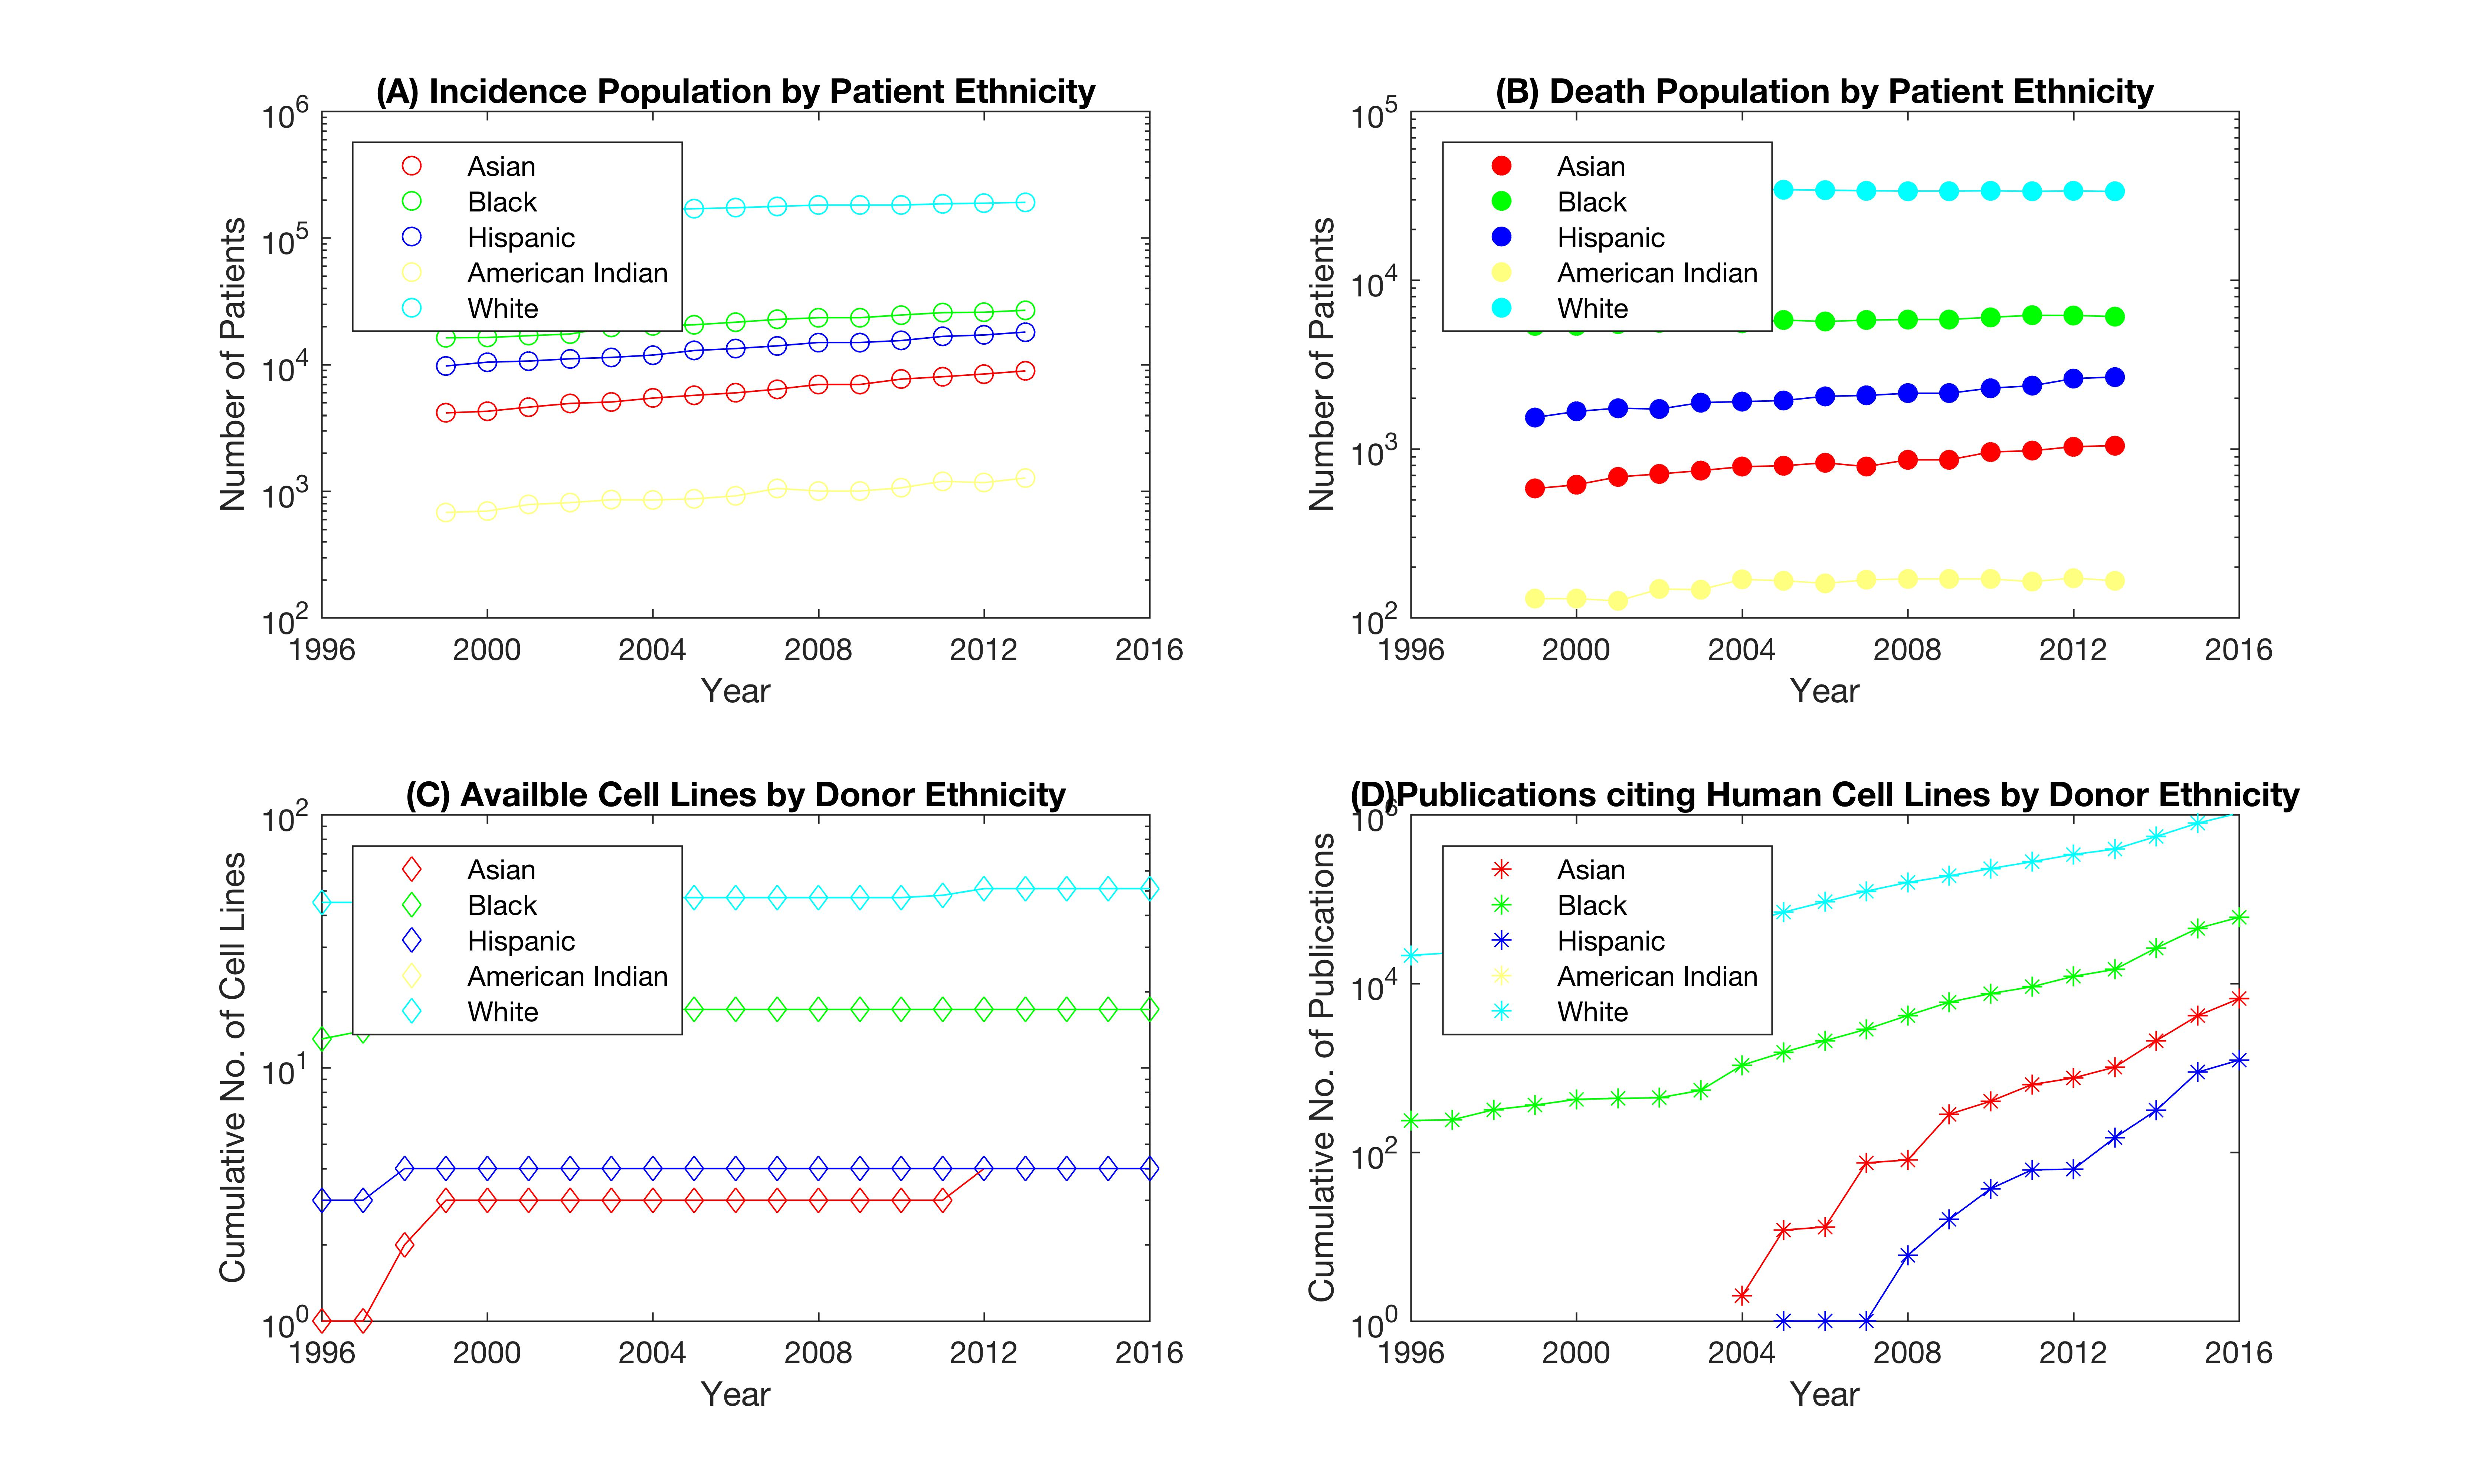
\includegraphics[width=1\columnwidth, trim = {10cm 0cm 10cm 0cm}, clip]{Figures/Timeline2x2.jpg}
\caption{\label{PS2} From top left: (A) Incidence of breast cancer from 1999 to 2013, grouped by ethnicity. (B) Death counts from breast cancer by ethnicity. (C) Proportion of available cell lines by ethnicity. (D) Proportion of citations of cell lines in published research, grouped by ethnicity.}% Demographic representation in available cell lines, publication and patents as compared to the death counts for breast cancer.}
\end{figure}

The breast cancer patient population includes all ethnic groups. Sorting the fraction each group comprises by the incidence number shows the incidence rate is in line with the population sizes: White, Black, Hispanic, Asian and Native American (Figure 2A). Matching the trend, the death population shows the same order from most populus to least (Figure 2B). Given that esearch is limited by resources and time, it is not surprising that the breast cancer cell line bank composition reflects the incidence and death population proportions (Figure 2C). Of the 154 cell lines available, 50\%, 78 cell lines were formed from donors of unknown ethnicity. Of breast cancer cell lines with known donor ethnicity, 51 were from White donors, 17 from Black donors, 4 Hispanic, 4 Asian, and none from Native American donors.

Understanding the importance of standards, reproducibility and the legacy of scientific research, we expect to observe a bias in the publication record toward available cell lines. This would mean cell lines donated by white patients should be the most cited lines in research. Of the more than 1.2 million publications citing a cell line, 1.0 million cited a cell line donated by white patients, 60k cited a line from a black patient, 6k cited a line an Asian patient, 1k cited Hispanic cell lines and none cited a cell lines from a Native Americans (none are available; Figure 2D).

How does the fraction of women in the incidence population compare to publications that cite a breast cancer cell line donated by a white woman? Since 1999, the fraction of white women has been less than the fraction of cell lines donated by white women. That is, cell lines over-represent white eomwn by more than 15\% overall and nearly 19\% in 2013 (Figure 3A). Other ethnicites have remained under-represented by the same metric. The under-representation of Hispanics increased from 3\% to nearly 6\% in 2013. Perhaps worse, the trend against Hispanic representation in cited cell lines is greater when comparing the death population fraction.

\begin{figure}[h!]
\centering
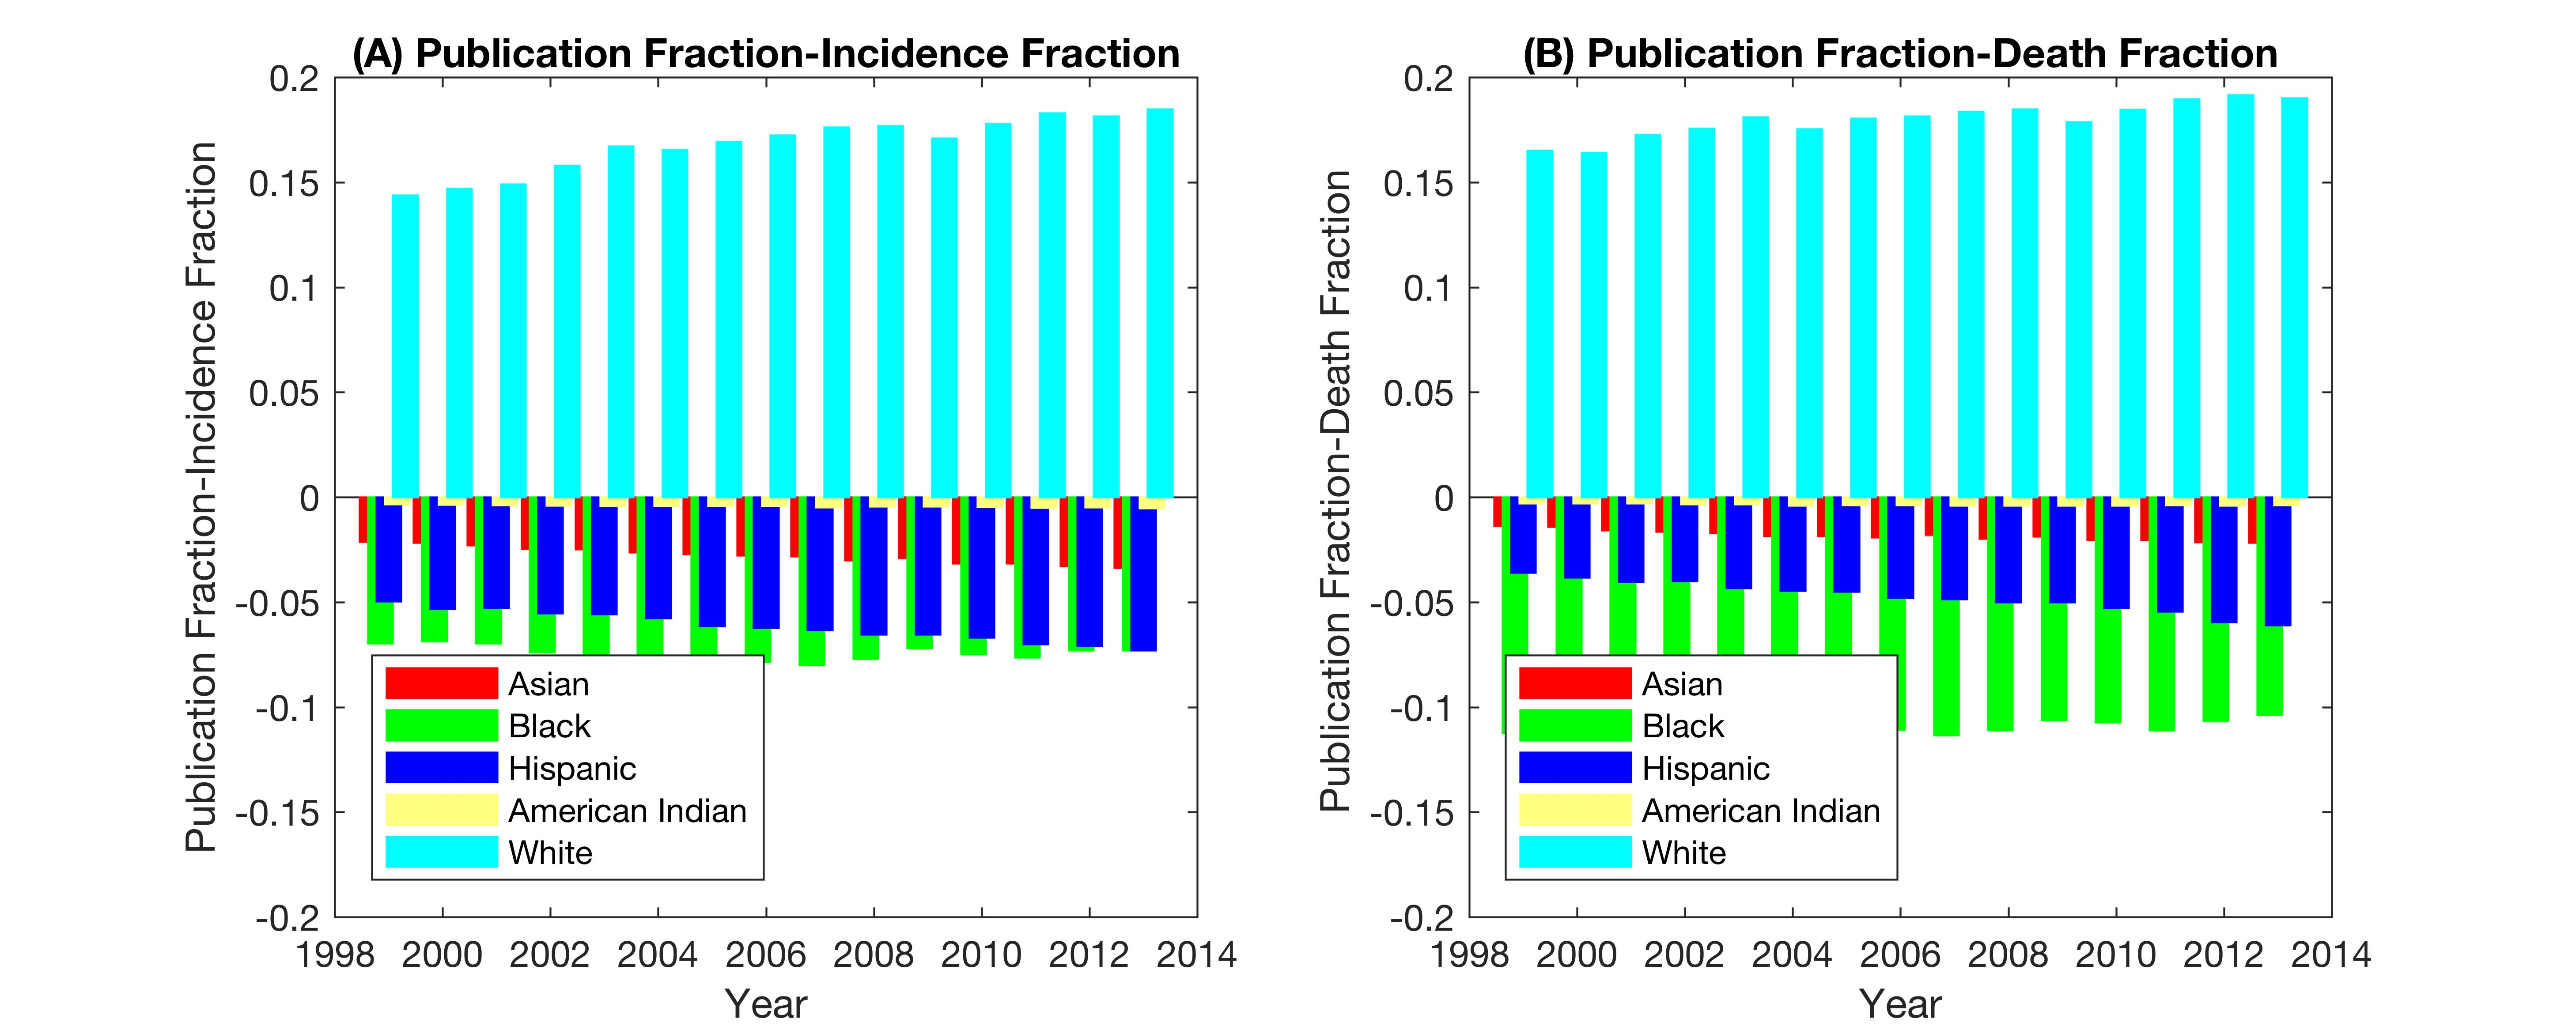
\includegraphics[width=1\columnwidth, trim = {10cm 0cm 10cm 0cm}, clip]{Figures/Bias.jpg}
\caption{\label{Bias} Representative bias in breast cancer medical research determined by comparing the fraction of each demographic group in the breast cancer death count to the proportional of cell lines cited in research publications and US patents from 1999 to 2013. White cell lines are proportionally over-represented, and getting morese, while Asian and Hispanic people are increasingly under-represented  and Black patients remain steadily under-represented. Patents are similarly biased against non-Whites, more biased against Blacks but with similar trends as research publications.}
\end{figure}

%Dependence on specific cell lines may influence the generalizability medical results. There are specific genetically sensitive targets which are prevalent in Black patients that are not included in cell models donated by Whites.

Research suggests black breast cancer patients present elevated risk for aggressive, intrinsic factors of breast cancer which adversely effect prognosis <NEED A CITATION>. The logical question is to what extent have black patients donated to cell lines used by medical researchers? And how well are these lines represented in published research and patents? Answers to these questions will determine the extent of under-representation, and requring corrective action to include cell lines that represent tumor sub-types causing the most morbidity.

%Raising the survival rate of black breast cancer patients to the national average requires critical review of socioeconomic-dependence of high-quality health care access and inclusive diagnostic techniques, without question \cite{shavers2003racial}. Failing to diagnosis at early stages, as well as faster growing, more aggressive tumor sub-types, disproportionately effect black patients \cite{batina2013variation}.

%The likely causes include societal, behavioral and biological factors, broadly categorized as extrinsic factors which are the responsibility of public policy and the individual, and intrinsic factors, such as genetics and cell structure within aggressive tumor sub-types, which are the responsibility of medical researchers to consider in designing fundamental research studies \cite{reding2012examination, brennan2012there}. 

%Research supports black breast cancer patients present elevated risk for aggressive, intrinsic factors of breast cancer which adversely effect prognosis. The next logical question is to what extent have black patients donated to cell lines used by medical researchers, and then, how well these lines are represented in published research and patents. The purpose of asking these questions is to determine any extent to under-representation, allowing for corrective action to simply include cell lines which represent the aggressive tumor sub-types causing the most morbidity. Data-driven retrospectives on disease burden and treatment effectiveness have been used in the past to guide medical research funding and health policy decisions towards the most productive population-level outcomes \cite{kim2016cancer}. 

The long term consequences of medical research into groups most represented in available and used cell lines have the serious implications in medical research. Targeted breast cancer therapies and preventative screening strategies that are sensitive to various tumors would help absolve demographic inequalities in breast cancer research and treatment \cite{batina2013variation}. Cell lines are a critical tool for developing medical treatments and their use use should be equitable to morbidity.% ``Human cancer in a test tube'' provides a standard for genotypic and phenotypic stability. 

%The next steps in breast cancer research characterizes the many sub-types of breast cancer as unique pathologies, relying on specific traits of the tumor and the patient's genetics to make decisions regarding treatment options. As the medical community pivots towards personalizing care based on genetic markers, we reflect on the inertia of breast cancer research. After acknowledging new genomic techniques change how we group patients, lets consider past use of ethnic groups. Before gene sequencing became widely available, the CDC grouped the US breast cancer patient population by ethnicity, to identify if and who was left out of improving health care options. The purpose being to expand healthy lifestyle choices, public awareness campaigns, diagnostics, and treatment options to include non-majority considerations. Cell model breast cancer research has developed tool to study non-majority ethnicities in the patient population, with the notable exception of Native Americans. Reliance on a select subset of these tool as standards to study breast cancer perpetuated the bias. An emphasis on genetics and tumor sub-types offers the possibility to refine the vocabulary used to group breast cancer patients, targeting differences in disease treatment option are able to directly address. 

\bibliographystyle{unsrt}
\bibliography{refs}


\end{document}
